\chapter{State of the Art}
\label{cha:state_of_the_art}

\todo{Add chapter introduction}

\section{Analysis of and Contributions to the C\&M Literature}

\todo{Do}

% \textit{In this chapter the (about 3 (BT) / 6 (MT)) publications with a high relevance for the thesis are described. Publications which do have no or only a weak relationship with the thesis should not be part of this chapter.}

% \section{Analysis of and Contributions to the C\&M LITERATURE}
% \label{sec:cm_literature}
% \textit{The C\&M LITERATURE is the source and destination of all literature work at C\&M}.

% \begin{figure}[bth]
%     \centering
%     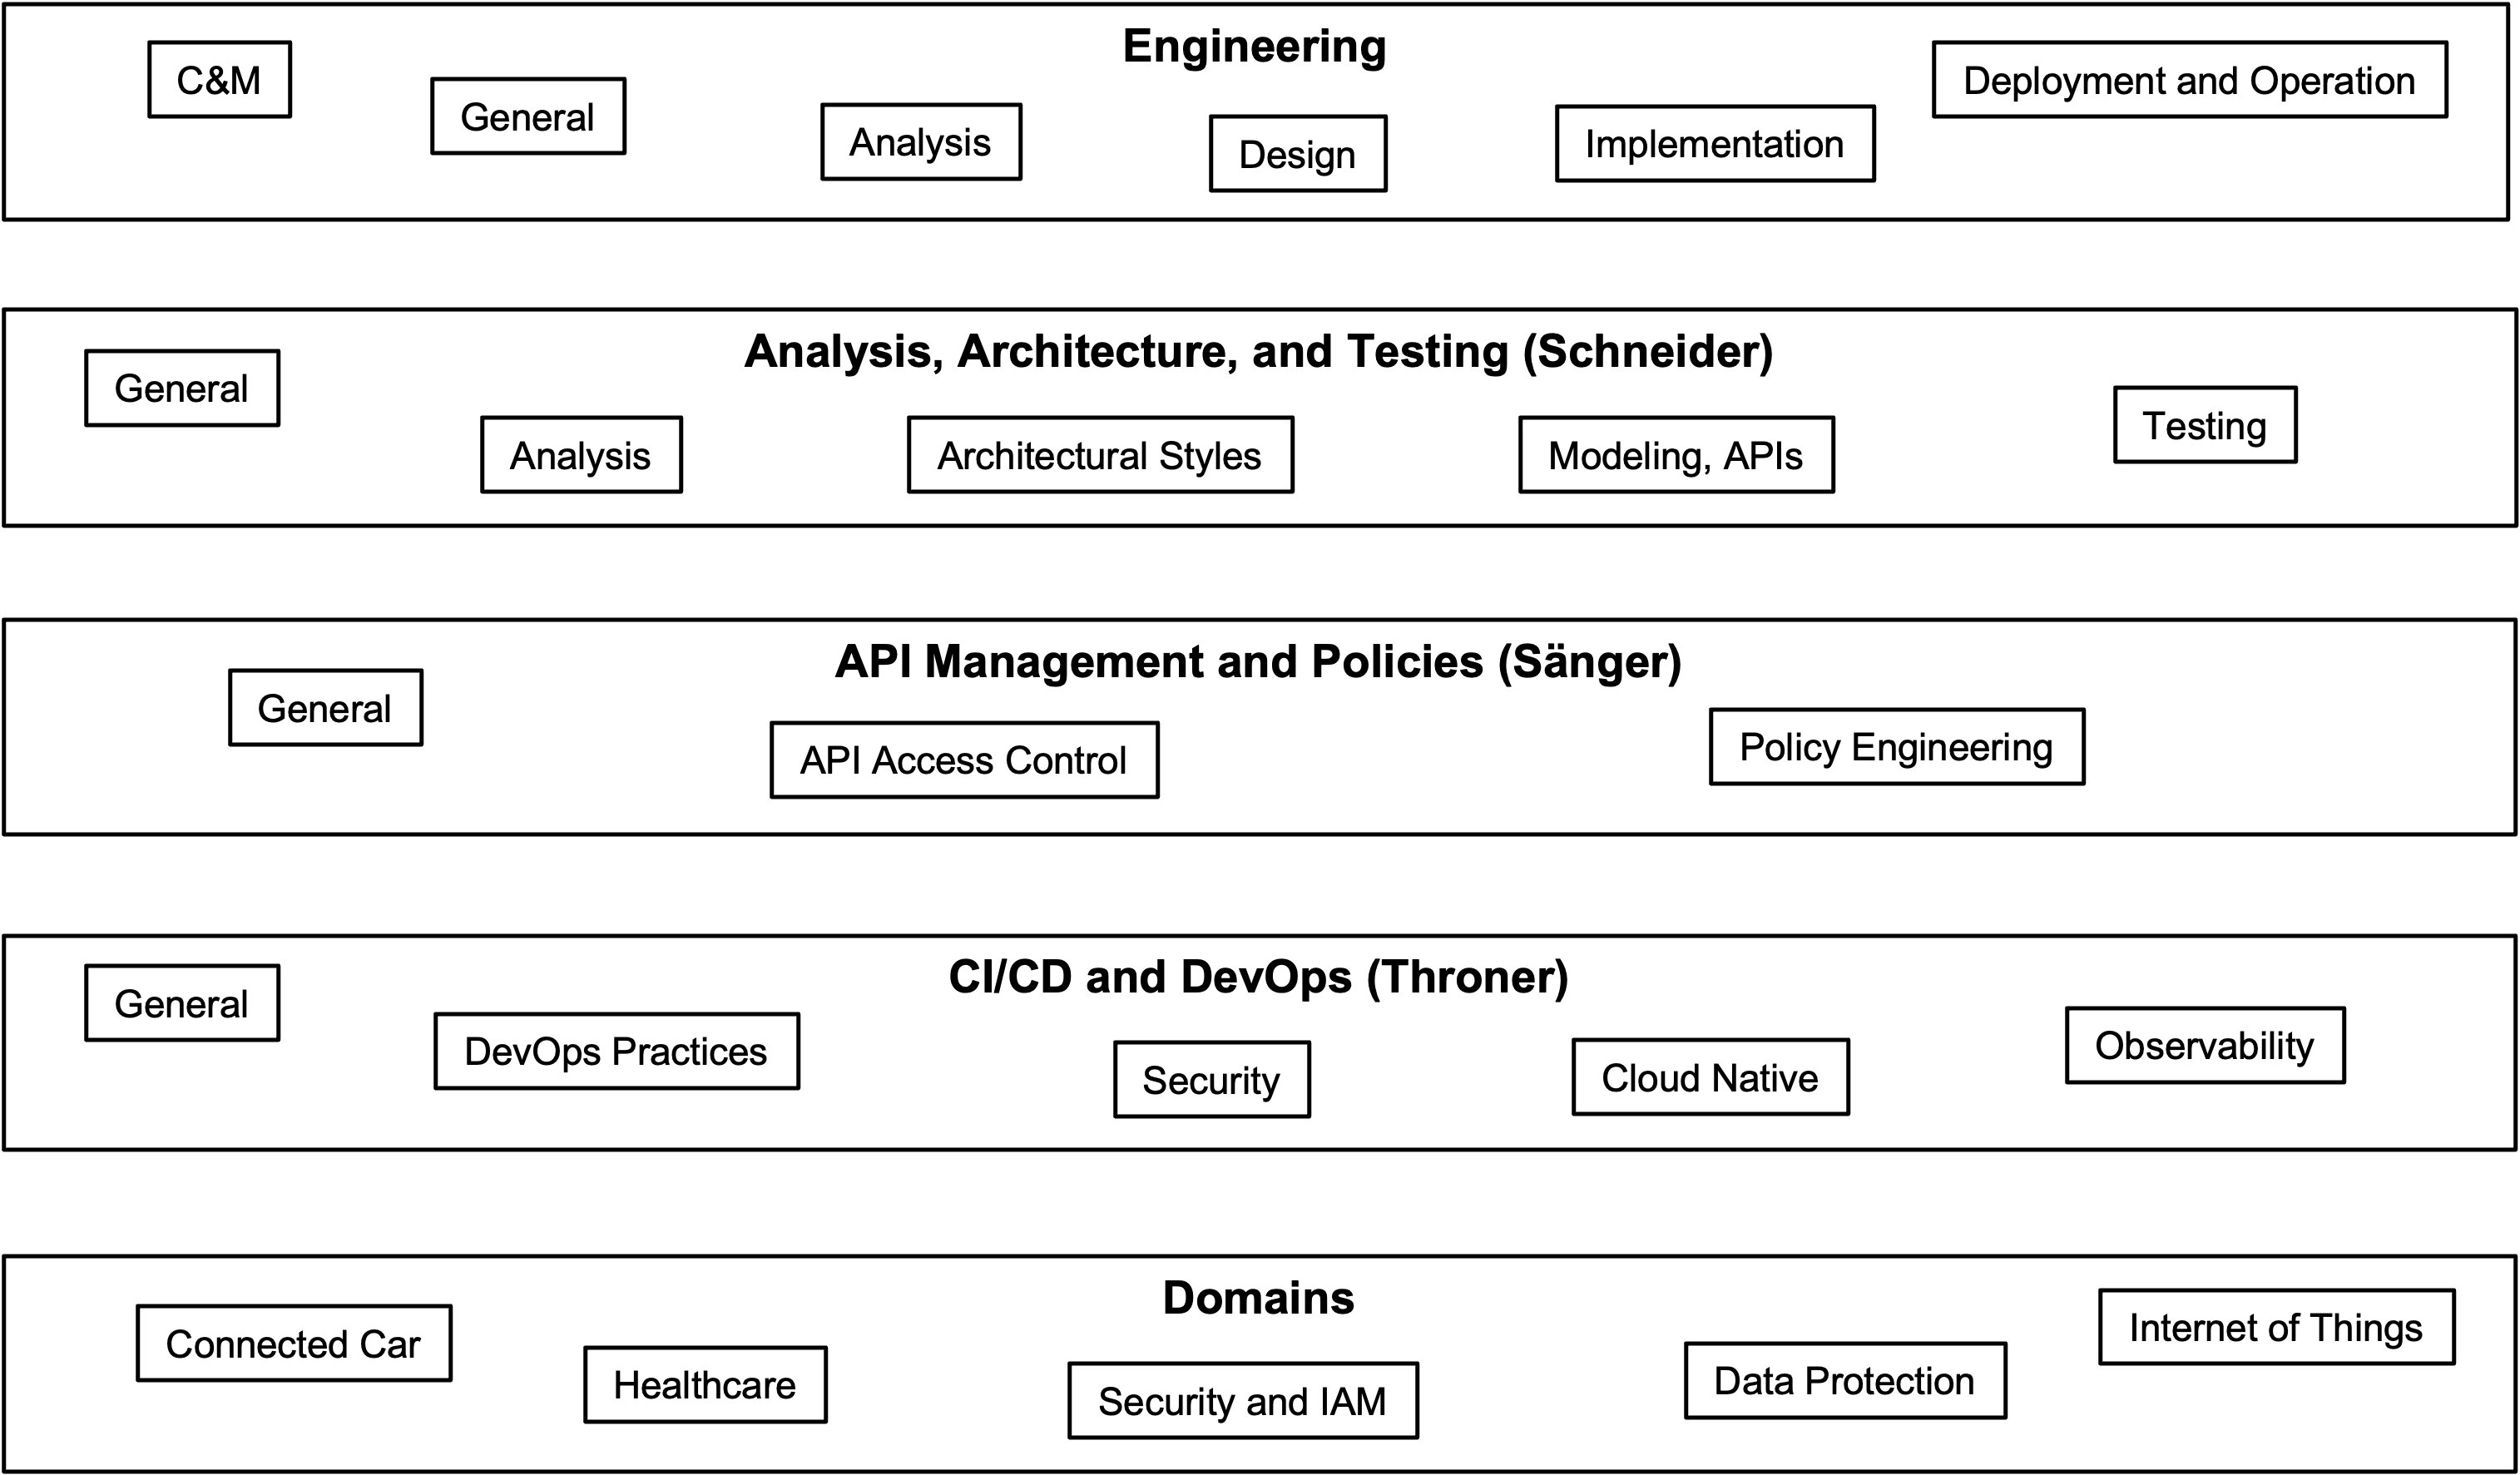
\includegraphics[width=\linewidth]{figures/structure}
%     \caption{Categories and Subcategories}
%     \label{fig:categories_subcategories}
% \end{figure}  

% \textit{The categorization is achieved by writing the index of the publication nearby the corresponding box of Figure \ref{fig:categories_subcategories}. 
% In this specific case, a publication \cite{Ev03} grouped into the subcategory ``Software Engineering - Analysis and Design'' and a publication [NN21] grouped into the subcategory ``IoT - Tasking'' are part of the state of the art of this thesis. A white box indicates that a publication and the subcategory already exists whereas a grey box and bold text emphasize a new publication and subcategory. The concrete steps to create the first figure of Chapter 3 in a BT/MT thesis are as follows:}
% \begin{enumerate}
% \item{The slide ``Categories and Subcategories'' of the PowerPoint file stored in the folder
% \url{\\\\sccfs.scc.kit.edu\\OE\\TM\\VR\\Mitglieder\\3-4.Literature} should be copied into the figures file of the BT/MT thesis.}
% \item{For the extension of this figure, the boxes used in the slide ''Categories and Subcategories'' of the PowerPoint file stored in the folder \url{\\\\sccfs.scc.kit.edu\\OE\\TM\\VR\\Mitglieder\\3.FORSCHUNG_PROJEKTE\\2-1.Working_Folder_Templates\\BTMT_Name} should be used.}
% \item{The figure in the BT/MT thesis should be titled ``Categorization of the Relevant Publications''.}
% \end{enumerate}
% \textit{
% For each publication, the (EXISTing or to be CHANGEd or to be CREATEd) C\&M LITERATURE entry for this publication is introduced in the following subsections. The publication \cite{Ev03} serves as the example of an EXISTing publication and the publication [NN21] serves as a new (i.e., to be CREATEd) publication. The publications are arranged according to the structure of the C\&M LITERATURE (i.e., ``Software Engineering'' followed by ``Microservices and APIs'' followed by ...).}

% \subsection{Domain-Driven Design: Tackling Complexity in the Heart of Software \cite{Ev03}}
% This is the textbook on Domain-Driven Design (DDD) written by the DDD founder, Eric Evans. Core parts covered by this textbook can be found in those parts of the WASA course units \cite{CM-W-WAS} dealing with the design of web applications. It should be noticed that Evans developed the DDD concept in 2003 independently from the microservices which only came up about ten years later (for this reason the textbook is not grouped into this category).

% Status: EXIST (the text is adopted from the C\&M LITERATURE (<Date>))

% \subsection{<Title of the Second Publication> <Index>}
% Description of the publication's content and relevance for C\&M

% Status: CREATE (the publication should become part of the  C\&M LITERATURE (<Date>))

% \subsection{<Title of the Third Publication> <Index>}
% ...

% \textit{In the following sections, the 1 to 2 (BT) / 2 to 4 (MT) publications which have the highest influence on the solution worked out in this thesis are described in more detail (about 2 pages). The focus of the description should be set on the relationship of these publications to the thesis.}

% \section{Author(s): Title of the Most Relevant Publication}
% \label{sec:index_of_the literature1}

% \section{Author(s): Title of the Second Most Relevant Publication}
% \label{sec:index_of_the literature2}